\begin{frame}
	\frametitle{O problema}
\begin{figure}[h]
	\caption{Obtos no trânsito de 2004 a 2015}
	\centering
	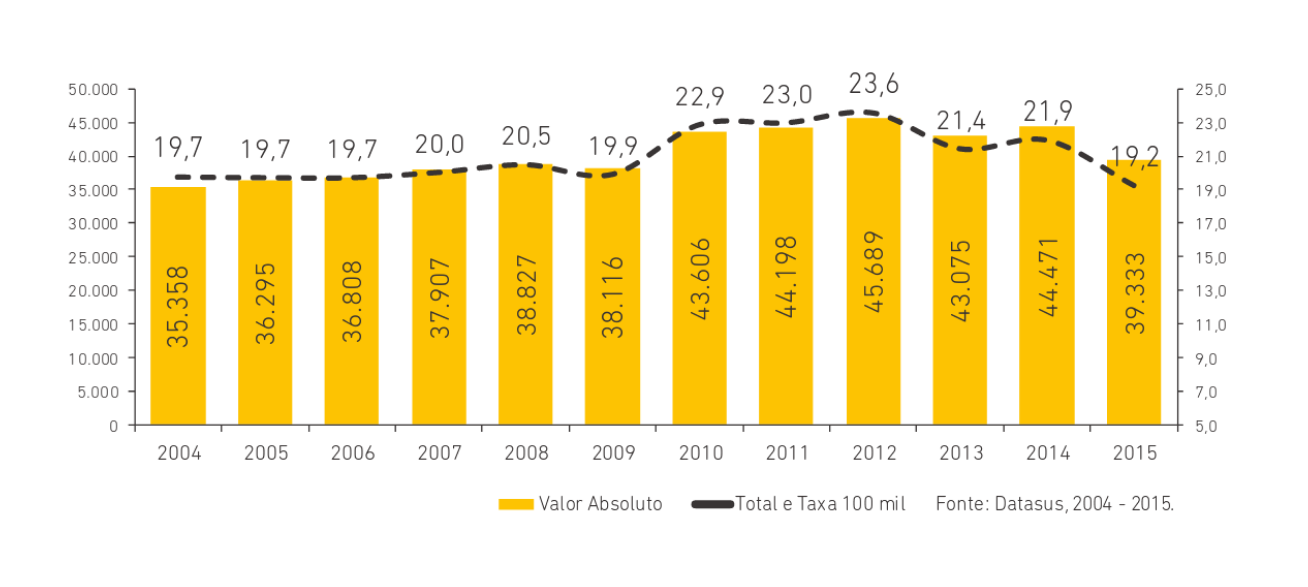
\includegraphics[width=1\textwidth]{imagens/obto}
	\end{figure}
\end{frame}

\begin{frame}
	\frametitle{O problema \textit{continuação}}
\begin{figure}[h]
	\caption{Vitimas não fatais no trânsito de 2004 a 2015}
	\centering
	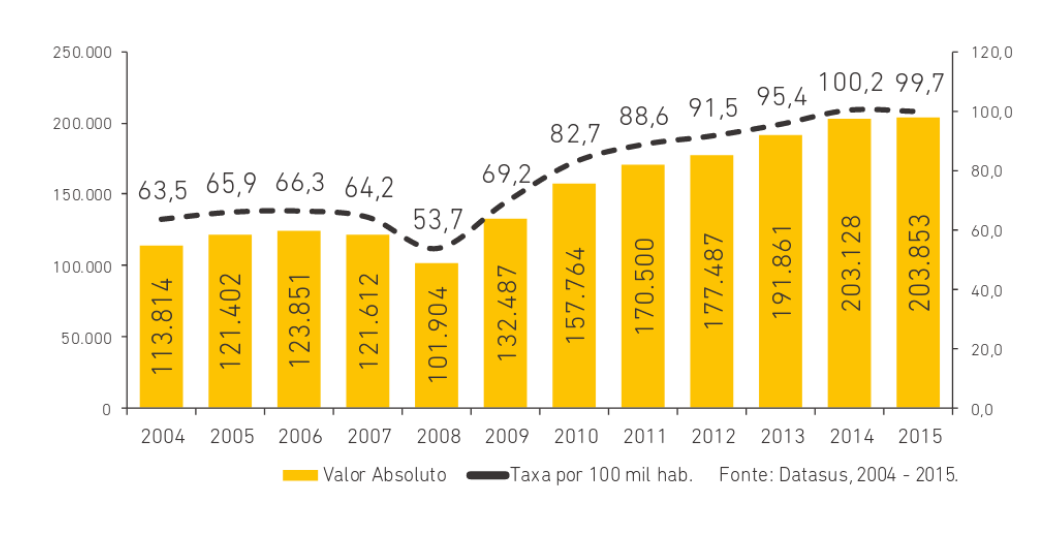
\includegraphics[width=1\textwidth]{imagens/ferido}
	\end{figure}
\end{frame}

\begin{frame}
	\frametitle{Efeitos do problema}
	Em 2015, acidentes relacionados ao trânsito chegou ao 
	10º lugar, no mundo, como maior caso de obtos;
	Gerando gastos de R\$ 19 Bilhões/ano para o Brasil\cite{ambev}.
\end{frame}

\begin{frame}
	\frametitle{Soluções Empregadas Atualmente (Brasil)}
	\begin{itemize}[<+->]
		\item Lei seca;
		\item Cinto de segurança;
		\item Cadeirinha infantil;
		\item Capacete;
		\item Regulametação e fiscalização de velocidadde máxima;
		\item \textbf{Câmeras de monitoramento}.
 	\end{itemize}
\end{frame}